\documentclass[a4paper]{article} %format de la feuille + type de document https://en.wikibooks.org/wiki/LaTeX/Document_Structure#Document_classes
%packages nécessaire pour nos besoins
\usepackage[utf8]{inputenc}
\usepackage[T1]{fontenc}
\usepackage[english,french]{babel}
\usepackage{amsmath}
\usepackage{amssymb,amsfonts,textcomp}
\usepackage{color}
\usepackage{array}
\usepackage{hhline}
\usepackage{hyperref}
\usepackage[pdftex]{graphicx}
\usepackage{sectsty}
\usepackage{tcolorbox}
\usepackage{textcomp}
\usepackage{courier}
\usepackage[font={small,it}]{caption}
\usepackage{float}
\usepackage{graphicx}
\usepackage{caption}
\usepackage{tabularx}
\usepackage{multirow}% http://ctan.org/pkg/multirow
\usepackage{tikz}
\usepackage[top=15mm,bottom=20mm,right=50mm,left=50mm]{geometry} 
\usepackage[export]{adjustbox}


%Définition des couleurs
\definecolor{havelockBlue}{rgb}{0.004, 0.42, 0.73}
\definecolor{Monokaimagenta}{rgb}{0.86,0.08,0.24}

%utilisation de la couleur définie avant
%toutes les sections auront cette couleur
\sectionfont{\color{havelockBlue}}
%\subsectionfont{\color{havelockBlue}}
%début du document
\begin{document}

\renewcommand{\labelitemi}{$\bullet$}
\renewcommand{\labelitemii}{$\cdot$}
\renewcommand{\labelitemiii}{$\diamond$}
\renewcommand{\labelitemiv}{$\ast$}

%début d'un titre
\begin{titlepage}
            %centre les éléments
	\centering
	
	{\scshape\LARGE \color{Monokaimagenta} Laboratoire \\  \par}
	
	%espace vertical de 1 mms
	\vspace{1cm}
	
	{\Large\itshape Sven Rouvinez \& Johanna Melly\par}
	
	%http://www.personal.ceu.hu/tex/spacebox.htm
	\vfill
	Professeur\par
	%met le texte en gras 
	\textbf{Carlos Andrés Peña} \par% ajoute une ligne 
	\vspace{1cm}
	Assistant\par
	\textbf{Gaëtan Matthey}
	
	\vfill

            %affiche la date actuelle
	{\large \today\par}
	
%fin de la page de titre
\end{titlepage}

\section{Objectifs du laboratoire}
La réalisation simplifiée de la partie EXECUTE d'un processeur en ajoutant les opérations arithmétiques et logiques, ainsi que les shifts. Les blocs FETCH et DECODE du processeur PRODIS ainsi qu'un programme à exécuter sont fournis.

\section{Blocs Logisim}
Nous avons décidé de séparer les blocs afin de permettre une meilleure modularité et abstraction du système EXECUTE.\\
\paragraph{Résumé}
\begin{itemize}
    \item     EXECUTE
\end{itemize}
\subsection{Etape 1}
L'objectif de cette première étape était de relever un chronogramme, d'étudier la façon dont étaient générées les signaux dans le bloc DECODE, et d'expliquer les valeurs relevées dans les deux instructions ADD.
\subsubsection{Instructions fournies}
Un programme assembleur a été fourni pour cette étape, et l'objectif était d'en relever un chronogramme dont les signaux étaient spécifiés dans la donnée.
Le programme assembleur est le suivant:\medskip \\ 
\begin{center}
\begin{tabular}{|c|c|c|c|}
    \hline
    MOV  & Rd & Rn   & Rm  \\
    \hline
    MOV  & r0 & \#3  &     \\
    \hline
    MOV  & r2 & r0   &     \\
    \hline
    ADD  & r3 & r2   & \#7 \\
    \hline
    ADD  & r5 & r3   & r0  \\
    \hline
    AND  & r3 & r5   &     \\
    \hline
    LSL  & r1 & r5   & \#2 \\
    \hline
    SUB  & r0 & r3   & r1  \\
    \hline
\end{tabular}
\end{center}

Légende des instructions:
\begin{itemize}
    \item \textbf{MOV} Move
    \item \textbf{ADD} Addition
    \item \textbf{AND} Opération logique "et"
    \item \textbf{LSL} Shift logique à gauche
    \item \textbf{SUB} Soustraction    
\end{itemize}
\medskip
Voici les valeurs présentes dans chaque registre au fil des instructions:
\begin{enumerate}
    \item r0 $\leftarrow$ 0x0003
    \item r2 $\leftarrow$ 0x0003
    \item r3 $\leftarrow$ 0x000a
    \item r5 $\leftarrow$ 0x000d
    \item r3 $\leftarrow$ 0x0000
    \item r1 $\leftarrow$ 0x0d00
    \item r0 $\leftarrow$ 0xf300 (à vérifier)
\end{enumerate}
\subsubsection{Chronogramme}
\begin{figure}[H]
    \centering
    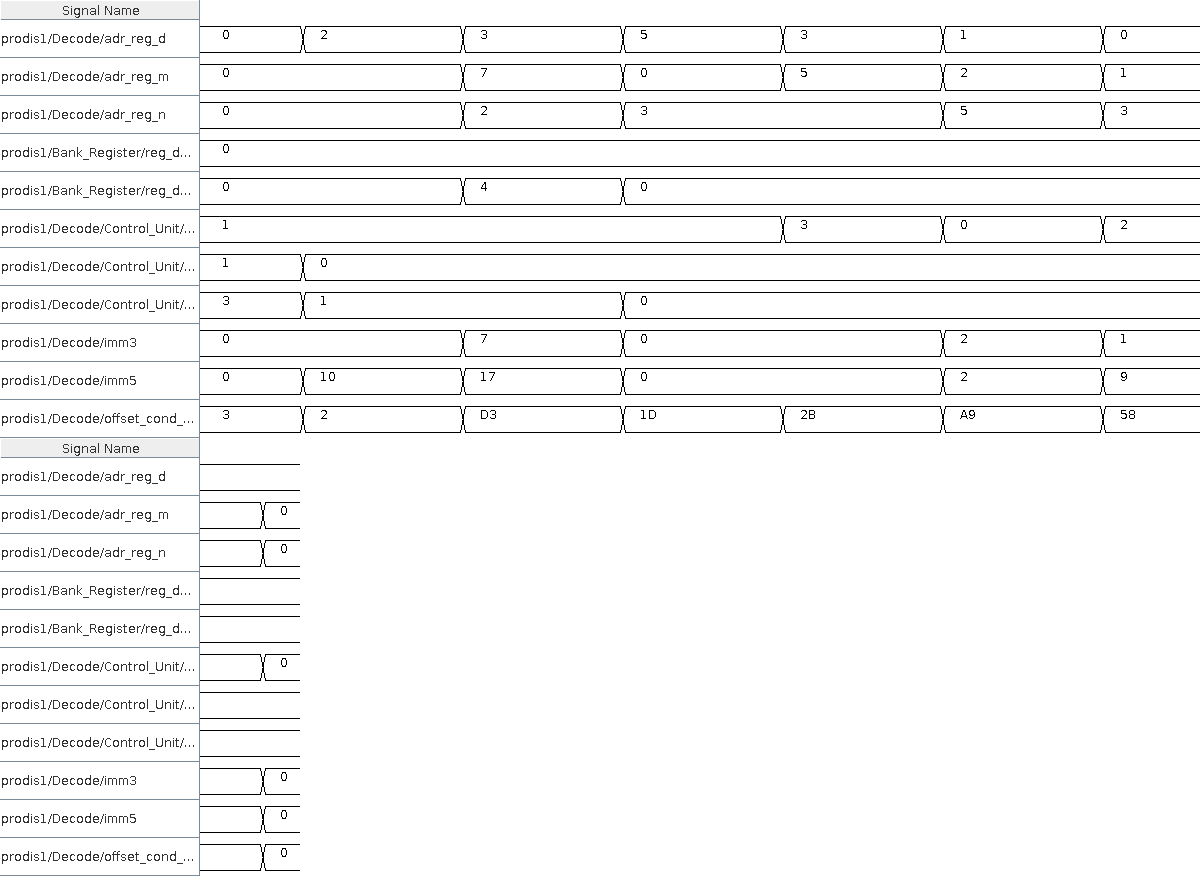
\includegraphics[width=1\textwidth]{src/CHRONO_ETAPE1.png}
    \captionof{figure}{Chronogramme}
    \label{fig:Chronogramme}
\end{figure}

\subsection{Etape 2}
L'objectif de cette étape était de réaliser un circuit permettant de traiter les informations mentionnées dans l'étape 1.
Un bus d'instruction donne les informations nécessaires au fonctionnement du bloc EXECUTE (numéros de registres, type d'opérations à faire, opérandes à utiliser). Le format de ces information est sur 23 bits et se présente comme suit: \medskip \\
\begin{itemize}
\item{[0-2] = sel\_op\_shift}
    \subitem 000: Bypass du bloc
    \subitem 001: Operand 1 shift arithmétique à droite avec Operand 2
    \subitem 010: Operand 1 shift logique à gauche avec Operand 2
    \subitem 011: Operand 1 shift logique à droite avec Operand 2
    \subitem 100: Operand 1 shift rotatif à droite avec Operand 2
\item{[3-6] = sel\_op\_ali}
    \subitem 0000: Bypass du bloc (Operand 1 en sortie)
    \subitem 0001: Operand 1 + Operand 2
    \subitem 0010: Operand 1 - Operand 2
    \subitem 0011: Operand 1 AND Operand 2
    \subitem 0100: Operand 1 OR Operand 2
    \subitem 0101: Operand 1 XOR Operand 2
    \subitem 0110: NOT Operand 1
    \subitem 0111: Operand 1 AND (NOT Operand 2)
    \subitem 1000: Operand 1 * Operand 2
\item{[7-8] = sel\_operand\_2}
    \subitem 00: reg\_data\_out\_m
    \subitem 01: immediate3
    \subitem 10: not used
    \subitem 11: immediate8
\item{[9-10] = sel\_operand\_1}
    \subitem 00: reg\_data\_out\_n
    \subitem 01: 0x0000
    \subitem 10: Branch with link
    \subitem 11: not used
\end{itemize}
\subsubsection{Chronogramme}

\subsection{Etape 3}
L'objectif de cette partie était de modifier le circuit afin qu'il puisse traiter des informations supplémentaires précisées dans la donnée, à savoir:
\medskip
\begin{itemize}
    \item Shift logique à gauche, avec valeur immédiate
    \item Shift logique à gauche, avec valeur en registre
    \item Shift logique à droite, avec valeur immédiate
    \item Shift logique à droite, avec valeur en registre
    \item Opération logique AND
    \item Opération logique OR
    \item Opération logique XOR
    \item Opération logique NOT
    \item Addition avec valeur immédiate
    \item Addition avec valeur en registre
    \item Soustraction avec valeur immédiate
    \item Soustraction avec valeur en registre
\end{itemize}
\subsubsection{Chronogramme}
\section{Conclusion}
\end{document}